\chapter{Anexos}

El presente capítulo recopila la documentación complementaria del sistema de información farmacéutica \textit{Vitalis PharmaSys}. Se estructura en tres secciones fundamentales: la especificación formal de la Guía de Estilo y Sistema de Diseño (\textit{Clinical Precision UI}), el catálogo de mockups y prototipos visuales de la interfaz de usuario, y la arquitectura de plantillas Blade que articula la capa de presentación dentro del entorno de desarrollo Laravel.

\section{Guía de Estilo y Sistema de Diseño (Clinical Precision UI)}

Para garantizar una experiencia visual armónica, ergonómica y orientada a mitigar la carga cognitiva en entornos farmacéuticos de alta demanda, se diseñó e implementó el sistema de diseño \textit{Clinical Precision UI}. Esta especificación combina el minimalismo clínico moderno con principios rigurosos de accesibilidad digital conforme a las directrices WCAG AA (\textit{Web Content Accessibility Guidelines}).

\subsection{Principios Rectores del Diseño}
La identidad visual del sistema se cimenta sobre tres pilares de interacción:
\begin{enumerate}
    \item \textbf{Autoridad y Rigor Sanitario:} Empleo de contrastes tipográficos nítidos, bordes reactivos a la luz y jerarquías tabulares estrictas que suprimen la ambigüedad en la lectura de dosis, claves farmacéuticas y fechas de vencimiento.
    \item \textbf{Claridad y Enfoque Humano:} Uso de tonalidades azules y petróleo calmantes con radios de curvatura suaves que disminuyen la fatiga visual del personal durante jornadas operativas continuas.
    \item \textbf{Lienzo Extendido (Full-Canvas Workflow):} Supresión de barras laterales fijas pesadas (\textit{persistent sidebars}) en favor de un área de trabajo horizontal maximizada de 12 columnas fluidas, asistida por un menú lanzador de aplicaciones flotante (\textit{App Launcher}) de acceso rápido.
\end{enumerate}

\subsection{Paleta de Colores Institucional y Funcional}
La arquitectura cromática de \textit{Vitalis PharmaSys} distribuye roles jerárquicos entre colores estructurales, acentos de acción y estados semánticos sanitarios, como se especifica en la Tabla \ref{tab:paleta_colores}.

\begin{table}[H]
\centering
\caption{Paleta cromática formal del sistema de diseño \textit{Clinical Precision UI}.}
\label{tab:paleta_colores}
\renewcommand{\arraystretch}{1.25}
\begin{tabularx}{\textwidth}{|l|c|X|}
\hline
\rowcolor[HTML]{E5E9EB}
\textbf{Token de Color} & \textbf{Código Hex} & \textbf{Función y Aplicación en la Interfaz} \\ \hline
\textit{Deep Petroleum Navy} & \texttt{\#022B3A} & Color primario ancla. Encabezados principales, barras de navegación superior, tipografía de alta jerarquía y botones de acciones administrativas críticas. \\ \hline
\textit{Clinical Teal} & \texttt{\#1F7A8C} & Color secundario y acento de acción. Botones primarios, enlaces activos, selectores interactivos y elementos de confirmación afirmativa. \\ \hline
\textit{Pale Sky} & \texttt{\#BFDBF7} & Acento atmosférico suave. Fondos de paneles visuales, tarjetas de autenticación, selecciones tipo píldora y bordes de realce sutil. \\ \hline
\textit{Canvas Base} & \texttt{\#F4F7F9} & Fondo general del lienzo de la aplicación. Proporciona contraste suave contra tarjetas blancas sin fatiga lumínica. \\ \hline
\textit{Surface Border} & \texttt{\#E8EFF5} & Divisores estructurales y bordes limpios para delimitación de tablas, tarjetas y contenedores modales. \\ \hline
\textit{Muted Slate} & \texttt{\#526E7D} & Tipografía secundaria, etiquetas descriptivas, textos auxiliares y metadatos con ratio de contraste accesible. \\ \hline
\textit{Pure White} & \texttt{\#FFFFFF} & Superficies de trabajo elevadas, contenedores modales, tarjetas de datos y fondos de tablas operativas. \\ \hline
\textit{Semantic Success} & \texttt{\#0F6B4F} & Indicadores de lote activo y producto en existencia (\textit{En Stock}). Complementado con fondo \texttt{\#E6F7F2}. \\ \hline
\textit{Semantic Warning} & \texttt{\#A05E03} & Alertas de existencias bajas próximas al umbral mínimo (\textit{Bajo Stock}). Complementado con fondo \texttt{\#FEF6E7}. \\ \hline
\textit{Semantic Danger} & \texttt{\#BA1A1A} & Alertas críticas de lotes vencidos o próximos a caducar ($<$30 días) y errores de validación. Fondo \texttt{\#FFDAD6}. \\ \hline
\end{tabularx}
\end{table}

\subsection{Sistema Tipográfico y Jerarquía Visual}
El sistema emplea una combinación armónica de dos familias tipográficas:
\begin{itemize}
    \item \textbf{Plus Jakarta Sans:} Fuente sans-serif de trazado geométrico contemporáneo y aperturas amplias, seleccionada como tipografía de interfaz principal debido a su legibilidad sobresaliente en tablas de datos densas, códigos de barras y números de lote.
    \item \textbf{Neuton:} Fuente serif editorial con remates sobrios, reservada para la marca institucional, logotipos de módulos y encabezados de bienvenida de alta jerarquía.
    \item \textbf{Cifras Tabulares (\texttt{tabular-nums}):} Todos los valores numéricos monetarios, cantidades de stock y fechas se renderizan mediante la propiedad CSS tipográfica de números tabulares, garantizando la alineación vertical exacta de columnas en reportes financieros y de almacén.
\end{itemize}

En la Tabla \ref{tab:escala_tipografica} se detalla la escala de tamaños, pesos e interlineados estandarizados.

\begin{table}[H]
\centering
\caption{Escala tipográfica estandarizada del sistema.}
\label{tab:escala_tipografica}
\renewcommand{\arraystretch}{1.2}
\begin{tabularx}{\textwidth}{|l|c|c|X|}
\hline
\rowcolor[HTML]{E5E9EB}
\textbf{Nivel Tipográfico} & \textbf{Tamaño} & \textbf{Peso} & \textbf{Caso de Uso Principal} \\ \hline
\textit{Display Hero} & 48px / 3rem & 800 (\textit{Bold}) & Encabezados principales del portal público y banner institucional. \\ \hline
\textit{Headline Large} & 32px / 2rem & 700 (\textit{Bold}) & Títulos de módulos principales (Dashboard, Ventas, Inventario). \\ \hline
\textit{Headline Medium} & 24px / 1.5rem & 600 (\textit{SemiBold}) & Subtítulos de sección y cabeceras de tarjetas analíticas. \\ \hline
\textit{Title Medium} & 16px / 1rem & 600 (\textit{SemiBold}) & Títulos de columnas en tablas y encabezados de modales. \\ \hline
\textit{Body Large} & 16px / 1rem & 400 (\textit{Regular}) & Párrafos introductorios y descripciones operativas. \\ \hline
\textit{Body Medium} & 14px / 0.875rem & 400 (\textit{Regular}) & Texto base de interfaz, celdas de tabla y formularios estándar. \\ \hline
\textit{Label Small} & 11px / 0.6875rem & 700 (\textit{Bold}) & Metadatos en mayúsculas, estados de lotes y badges semafóricos. \\ \hline
\end{tabularx}
\end{table}

\subsection{Retícula Espacial y Radios de Curvatura}
La maquetación visual se asienta sobre una retícula armónica fundamentada en incrementos de 8 puntos (espaciados de 8px, 16px, 24px, 32px y 48px). Asimismo, la jerarquía de elevación geométrica aplica radios de curvatura consistentes según el nivel del contenedor:
\begin{itemize}
    \item \textbf{Micro-elementos (\texttt{rounded-md} --- 6px a 8px):} Badges de lote, etiquetas de régimen sanitario y casillas de verificación.
    \item \textbf{Controles de Entrada (\texttt{rounded-lg} --- 10px a 12px):} Cajas de texto, listas desplegables y botones operativos.
    \item \textbf{Superficies y Tarjetas (\texttt{rounded-xl} --- 16px):} Paneles de métricas KPI, contenedores de tablas y resúmenes de venta.
    \item \textbf{Contenedores Maestros y Modales (\texttt{rounded-2xl} --- 20px a 24px):} Menú lanzador de aplicaciones (App Launcher) y diálogo de dispensación.
    \item \textbf{Indicadores de Píldora (\texttt{rounded-full} --- 9999px):} Buscador global superior y etiquetas de disponibilidad.
\end{itemize}

\section{Mockups y Prototipos de Interfaz de Usuario}

La arquitectura visual de \textit{Vitalis PharmaSys} fue concebida a partir de prototipos funcionales de alta fidelidad que modelan las pantallas clave tanto para la interacción del público en general como para la operación interna del personal químico-farmacéutico.

\subsection{Prototipo 1: Portal Público y Catálogo Digital Farmacéutico}
El portal público constituye el punto de contacto inicial con el usuario final. Dispone de un encabezado con información de guardia y farmacia de turno, un área principal (\textit{Hero}) orientada a la carga de recetas médicas electrónicas y exploración de medicamentos, categorías con conteo dinámico de productos, promociones destacadas y geolocalización de la sucursal central. En la Figura \ref{fig:anexo_portal_publico} se ilustra la composición integral de este prototipo.

\begin{figure}[H]
    \centering
    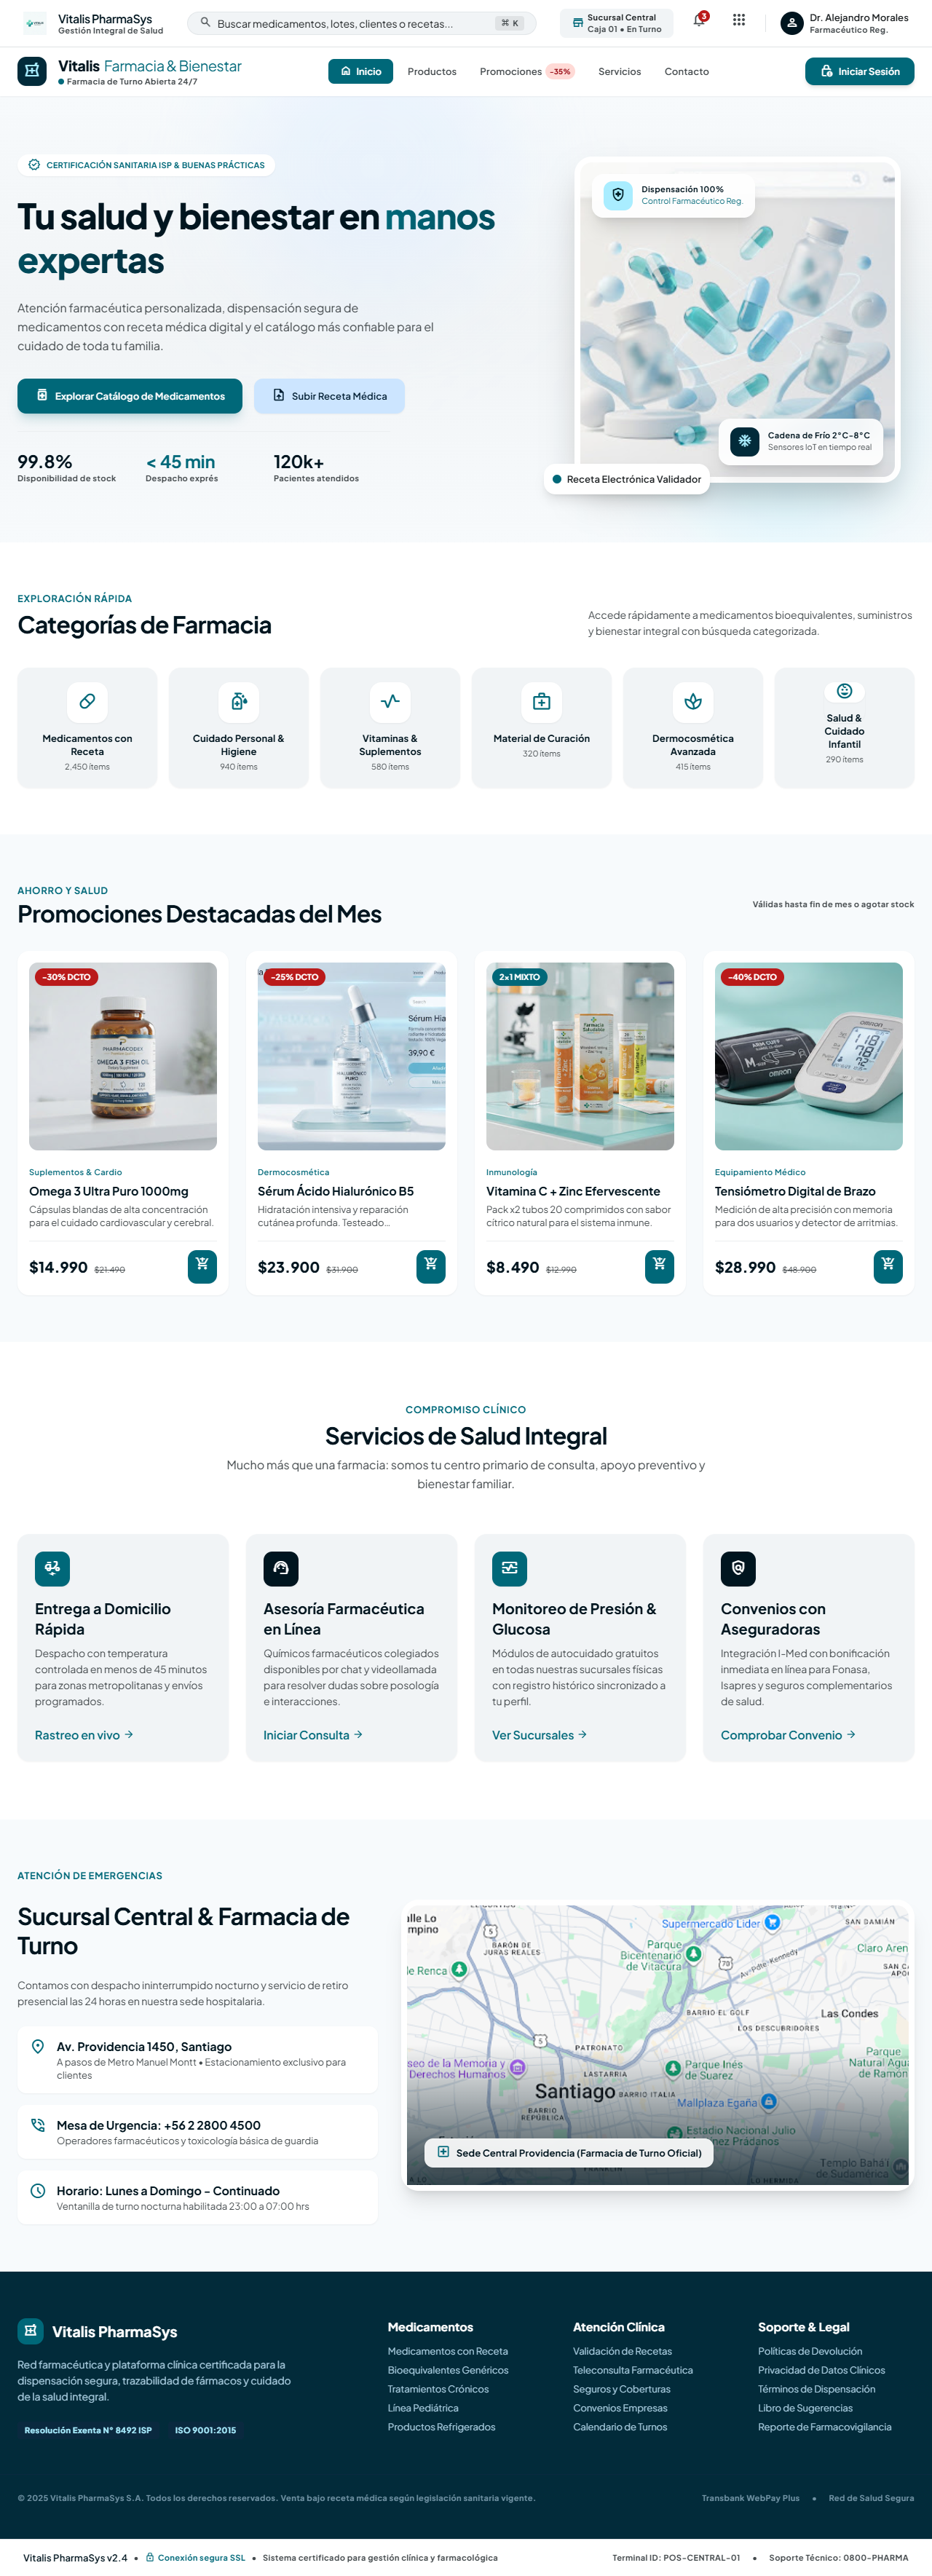
\includegraphics[width=0.92\textwidth]{imagenes/screen.png}
    \caption{Prototipo del portal público institucional y catálogo digital de medicamentos (\textit{Vitalis PharmaSys}).}
    \label{fig:anexo_portal_publico}
\end{figure}

Como se aprecia en la Figura \ref{fig:anexo_portal_publico}, la interfaz prioriza el acceso transparente a certificaciones sanitarias, trazabilidad de fármacos bajo cadena de frío ($2^\circ\text{C}$ a $8^\circ\text{C}$) y validación de prescripciones médicas, manteniendo una disposición visual libre de saturación publicitaria.

\subsection{Prototipo 2: Panel de Control Administrativo (Dashboard) y Trazabilidad de Lotes}
El panel operativo para regentes y dependientes farmacéuticos concentra los indicadores neurálgicos del establecimiento: importe de ventas del turno en curso, total de recetas retenidas y auditadas, alertas de medicamentos bajo punto de reorden y lotes con vencimiento próximo en ventana de 30 días con política FEFO. La Figura \ref{fig:mockup_dashboard_panel} describe la distribución modular de dicho panel.

\begin{figure}[H]
    \centering
    \fbox{
        \begin{minipage}{0.92\textwidth}
        \vspace{1.5cm}
        \centering
        \textbf{\large PANEL DE CONTROL ADMINISTRATIVO (DASHBOARD)}\\[0.3cm]
        \textit{Módulo Operativo de Monitoreo de Lotes, Existencias en Sala y Ventas del Turno}\\[0.5cm]
        \begin{tabular}{|c|c|c|c|}
            \hline
            \textbf{Ventas del Día} & \textbf{Recetas Médicas} & \textbf{Stock Crítico} & \textbf{Vencimientos (30 días)} \\
            \$ 1,420,500 & 84 validadas & 12 productos & 5 lotes (prioridad FEFO) \\ \hline
        \end{tabular}\\[0.8cm]
        \fbox{\parbox{0.85\textwidth}{\centering \textbf{Tabla Dinámica de Trazabilidad}: Medicamento, Lote Sanitario, Fecha Caducidad, Stock en Sala, Precio Unitario, Estado Semafórico y Acción de Dispensación Inmediata.}}\\[1.5cm]
        \end{minipage}
    }
    %\includegraphics[width=0.92\textwidth]{imagenes/mockup_dashboard.png}
    \caption{Esquema prototípico del panel de control farmacéutico y trazabilidad de lotes.}
    \label{fig:mockup_dashboard_panel}
\end{figure}

\subsection{Prototipo 3: Menú Lanzador de Aplicaciones (App Launcher 9 Puntos)}
Para optimizar el espacio de trabajo en pantalla y erradicar barras laterales invasivas, el sistema incorpora un componente modal flotante de 9 puntos (\textit{3x3 matrix}). Al ser accionado en la barra superior, despliega una matriz de navegación que permite transitar instantáneamente entre los módulos de Inventario, Ventas, Recetas, Pacientes, Arqueo de Caja, Reportes y Auditoría, tal como se esquematiza en la Figura \ref{fig:mockup_launcher}.

\begin{figure}[H]
    \centering
    \fbox{
        \begin{minipage}{0.75\textwidth}
        \vspace{1.0cm}
        \centering
        \textbf{\large LANZADOR GLOBAL DE MÓDULOS (APP LAUNCHER 3x3)}\\[0.3cm]
        \textit{Modal Flotante de Acceso Inmediato a Funcionalidades del Sistema}\\[0.6cm]
        \begin{tabular}{|c|c|c|}
            \hline
            [Dashboard] & [Inventario \& Lotes] & [Punto de Venta POS] \\ \hline
            [Recetas Médicas] & [Arqueo de Caja] & [Compras / Proveedores] \\ \hline
            [Kárdex / Movimientos] & [Reportes Financieros] & [Configuración / Roles] \\ \hline
        \end{tabular}\\[0.6cm]
        \footnotesize{Activación mediante botón con matriz geométrica en barra superior (dimensiones $340\text{px} \times 380\text{px}$).}\\[1.0cm]
        \end{minipage}
    }
    %\includegraphics[width=0.85\textwidth]{imagenes/mockup_launcher.png}
    \caption{Esquema conceptual del menú lanzador de aplicaciones (\textit{App Launcher}).}
    \label{fig:mockup_launcher}
\end{figure}

\subsection{Prototipo 4: Módulo de Acceso y Autenticación con Pantalla Dividida (Split-Screen)}
La pantalla de inicio de sesión implementa una composición dividida al 50\% en pantallas de escritorio. La columna izquierda presenta el panel institucional teñido en \textit{Pale Sky} (\texttt{\#BFDBF7}) con información de seguridad SSL y certificación sanitaria; la columna derecha aloja el formulario limpio de ingreso con campos para correo electrónico, clave de acceso, enlace de recuperación y botón primario en \textit{Clinical Teal} (\texttt{\#1F7A8C}), como se ilustra en la Figura \ref{fig:mockup_login_split}.

\begin{figure}[H]
    \centering
    \fbox{
        \begin{minipage}{0.88\textwidth}
        \vspace{1.2cm}
        \centering
        \textbf{\large PANTALLA DE ACCESO Y AUTENTICACIÓN (SPLIT-SCREEN 50/50)}\\[0.3cm]
        \textit{Estructura Visual con Panel de Garantía Sanitaria y Formulario Centrado}\\[0.5cm]
        \begin{tabular}{|p{0.42\textwidth}|p{0.42\textwidth}|}
            \hline
            \centering \textbf{Panel Visual Institucional} & \centering \textbf{Formulario de Ingreso} \tabularnewline
            - Fondo Pale Sky (\texttt{\#BFDBF7}) & - Caja de Correo Institucional \tabularnewline
            - Credenciales de Seguridad ISP & - Clave de Acceso Encriptada \tabularnewline
            - Declaración de Trazabilidad & - Casilla Recordar Sesión \tabularnewline
            - Acentos Geométricos Médicos & - Botón Primario: \textit{Iniciar Sesión} \tabularnewline
            \hline
        \end{tabular}\\[1.2cm]
        \end{minipage}
    }
    %\includegraphics[width=0.88\textwidth]{imagenes/mockup_login.png}
    \caption{Esquema estructural de la vista de autenticación dividida (\textit{Split-Screen}).}
    \label{fig:mockup_login_split}
\end{figure}

\section{Plantillas Blade y Arquitectura de Vistas}

La capa de presentación del sistema está construida bajo el motor de plantillas Blade de Laravel. Esta tecnología permite combinar sintaxis HTML5 limpia con estructuras de control optimizadas y directivas de herencia modular, compilando a código PHP nativo en caché para garantizar tiempos de respuesta ultrarrápidos.

\subsection{Estructura Jerárquica y Directivas Empleadas}
La arquitectura de vistas de \textit{Vitalis PharmaSys} sigue un patrón de herencia de doble nivel:
\begin{itemize}
    \item \texttt{@extends('layouts.app')}: Establece el diseño maestro que provee los metadatos HTML, enlaces de tipografías web (Plus Jakarta Sans y Neuton), inclusión de hojas de estilo compiladas mediante Vite (\texttt{@vite}), scripts de detección de modo oscuro/claro y la estructura del encabezado administrativo.
    \item \texttt{@section('content')} y \texttt{@yield('content')}: Definen las regiones dinámicas donde cada módulo hijo inyecta su contenido específico, evitando la duplicación de código de cabecera y pie de página.
    \item \texttt{@csrf}: Directiva de seguridad obligatoria en todos los formularios HTML que genera automáticamente un token criptográfico para neutralizar ataques de falsificación de peticiones en sitios cruzados (\textit{Cross-Site Request Forgery}).
    \item \texttt{@if / @else / @endif}: Control condicional de renderizado, empleado para alternar entre activos locales generados por Vite o el CDN de Tailwind CSS con configuración extendida autónoma.
\end{itemize}

\subsection{Plantilla 1: Layout Administrativo Principal (\texttt{layouts/app.blade.php})}
Este archivo gobierna la estructura visual de todas las pantallas protegidas del sistema. Contiene el encabezado con el buscador global tipo píldora, la identificación de la sucursal y caja activa, el alternador de tema claro/oscuro y el lanzador de aplicaciones de 9 puntos. En el Listado de Código \ref{lst:blade_layout_app} se presenta el fragmento arquitectónico representativo.

\begin{lstlisting}[language=HTML, caption={Estructura base del layout administrativo principal (\texttt{resources/views/layouts/app.blade.php}).}, label={lst:blade_layout_app}]
<!DOCTYPE html>
<html lang="es" class="scroll-smooth">
<head>
  <meta charset="utf-8">
  <meta name="viewport" content="width=device-width, initial-scale=1.0">
  <title>@yield('title', 'Vitalis PharmaSys — Panel de Gestión Farmacéutica')</title>

  <!-- Tipografias: Neuton & Plus Jakarta Sans -->
  <link href="https://fonts.googleapis.com/css2?family=Neuton:wght@400;700&family=Plus+Jakarta+Sans:wght@400;600;700;800&display=swap" rel="stylesheet">

  <!-- Script de deteccion de tema (Claro / Oscuro) -->
  <script>
    const theme = localStorage.getItem('theme');
    if (theme === 'dark') {
      document.documentElement.classList.add('dark');
    } else {
      document.documentElement.classList.remove('dark');
    }
  </script>

  <!-- Estilos Vite con Fallback de Contingencia -->
  @if (file_exists(public_path('build/manifest.json')) || file_exists(public_path('hot')))
    @vite(['resources/css/app.css', 'resources/js/app.js'])
  @else
    <script src="https://cdn.tailwindcss.com"></script>
    <link rel="stylesheet" href="{{ asset('css/custom.css') }}">
  @endif
</head>
<body class="bg-[#f4f7f9] dark:bg-[#08141d] text-[#022b3a] min-h-screen flex flex-col font-sans">

  <!-- Encabezado Superior Sticky con Buscador Global y Caja Activa -->
  <header class="w-full bg-white dark:bg-[#0b1a24] border-b border-[#e8eff5] h-16 sticky top-0 z-40">
    <div class="h-full px-6 flex items-center justify-between gap-4">
      <div class="flex items-center gap-3">
        <a href="{{ url('/dashboard') }}" class="font-brand font-bold text-xl text-[#022b3a]">
          PharmaSys
        </a>
        <span class="text-xs text-[#526e7d]">Sucursal Central • Caja 01</span>
      </div>
      
      <!-- Inyeccion Dinamica de Acciones de Cabecera -->
      <div class="flex items-center gap-3">
        @yield('header-actions')
      </div>
    </div>
  </header>

  <!-- Contenedor de Contenido Principal -->
  <main class="flex-1 w-full max-w-7xl mx-auto px-4 py-6">
    @yield('content')
  </main>
</body>
</html>
\end{lstlisting}

\subsection{Plantilla 2: Panel de Control y Trazabilidad (\texttt{dashboard.blade.php})}
La plantilla del panel de control demuestra la integración de directivas de herencia modular y el despliegue de datos operacionales en tiempo real. En el Listado de Código \ref{lst:blade_dashboard} se muestra la composición de las tarjetas de métricas analíticas y la cabecera de la tabla de lotes con fechas de expiración.

\begin{lstlisting}[language=HTML, caption={Fragmento de métricas y trazabilidad en \texttt{resources/views/dashboard.blade.php}.}, label={lst:blade_dashboard}]
@extends('layouts.app')

@section('title', 'Dashboard — Vitalis PharmaSys')

@section('content')
<div class="bg-white dark:bg-[#0d1e2b] border border-[#e8eff5] rounded-2xl p-6 shadow-clinical-sm">
  
  <!-- Titulo y Accion de Nueva Dispensacion -->
  <div class="flex items-center justify-between pb-6 mb-6 border-b border-[#e8eff5]">
    <div>
      <h1 class="font-brand font-bold text-2xl text-[#022b3a] dark:text-white">
        Panel de Control Farmacéutico
      </h1>
      <p class="text-xs text-[#526e7d]">Dispensación y trazabilidad de lotes en tiempo real.</p>
    </div>
    <a href="{{ url('/ventas/create') }}" class="px-4 py-2 rounded-xl text-sm font-semibold bg-[#1f7a8c] text-white">
      Nueva Dispensación
    </a>
  </div>

  <!-- Rejilla de Indicadores Operativos (KPI) -->
  <div class="grid grid-cols-1 sm:grid-cols-2 lg:grid-cols-4 gap-4 mb-8">
    <div class="p-4 rounded-xl bg-[#f4f7f9] border border-[#e8eff5]">
      <span class="text-xs font-semibold text-[#526e7d]">Ventas del Día</span>
      <span class="text-2xl font-bold text-[#022b3a] tabular-nums block">$ 1,420,500</span>
      <span class="text-[11px] text-[#0f6b4f] font-semibold">128 comprobantes</span>
    </div>
    <div class="p-4 rounded-xl bg-[#f4f7f9] border border-[#e8eff5]">
      <span class="text-xs font-semibold text-[#526e7d]">Lotes Críticos (30 días)</span>
      <span class="text-2xl font-bold text-[#ba1a1a] tabular-nums block">5</span>
      <span class="text-[11px] text-[#ba1a1a] font-semibold">Prioridad de rotación FEFO</span>
    </div>
  </div>

  <!-- Tabla de Trazabilidad Sanitaria de Lotes -->
  <div class="overflow-x-auto rounded-xl border border-[#e8eff5]">
    <table class="w-full text-left text-xs">
      <thead class="bg-[#f4f7f9] text-[#526e7d] uppercase font-bold">
        <tr>
          <th class="py-3 px-4">Medicamento / Presentación</th>
          <th class="py-3 px-4">Lote Sanitario</th>
          <th class="py-3 px-4">Caducidad</th>
          <th class="py-3 px-4">Stock Sala</th>
          <th class="py-3 px-4">Estado</th>
        </tr>
      </thead>
      <tbody class="divide-y divide-[#e8eff5]">
        <!-- Registro con Semaforizacion Verde (En Stock) -->
        <tr>
          <td class="py-3 px-4 font-bold text-[#022b3a]">Amoxicilina + Ác. Clavulánico</td>
          <td class="py-3 px-4 font-mono">AMX-2026-09</td>
          <td class="py-3 px-4 tabular-nums">15/09/2027</td>
          <td class="py-3 px-4 tabular-nums">45 unidades</td>
          <td class="py-3 px-4">
            <span class="px-2 py-0.5 rounded-full text-[10px] font-bold bg-[#e6f7f2] text-[#0f6b4f]">
              En Stock
            </span>
          </td>
        </tr>
      </tbody>
    </table>
  </div>
</div>
@endsection
\end{lstlisting}

\subsection{Plantilla 3: Autenticación con Pantalla Dividida (\texttt{auth/login.blade.php})}
La vista de autenticación ilustra la implementación de mecanismos de protección criptográfica y organización visual adaptativa mediante Tailwind CSS, tal como se expone en el Listado de Código \ref{lst:blade_login}.

\begin{lstlisting}[language=HTML, caption={Implementación de la vista de acceso (\texttt{resources/views/auth/login.blade.php}).}, label={lst:blade_login}]
<!DOCTYPE html>
<html lang="es">
<head>
  <meta charset="utf-8">
  <title>Iniciar Sesión — Vitalis PharmaSys</title>
  @vite(['resources/css/app.css', 'resources/js/app.js'])
</head>
<body class="bg-[#f4f7f9] min-h-screen flex items-center justify-center p-6 font-sans">
  
  <!-- Contenedor Maestro Split-Screen -->
  <div class="w-full max-w-4xl bg-white border border-[#e8eff5] rounded-2xl shadow-clinical-lg grid grid-cols-1 lg:grid-cols-12 overflow-hidden">
    
    <!-- Columna Izquierda: Brand Panel en Pale Sky (#BFDBF7) -->
    <div class="lg:col-span-5 bg-[#bfdbf7] p-8 flex flex-col justify-between border-r border-[#e8eff5]">
      <div>
        <h2 class="font-brand font-bold text-2xl text-[#022b3a]">Vitalis PharmaSys</h2>
        <p class="text-xs text-[#022b3a]/80 mt-2">Plataforma clínica certificada para gestión de dispensación y recetas.</p>
      </div>
      <span class="text-[11px] text-[#022b3a]/70">Conexión Segura SSL • Cumplimiento COFEPRIS / ISP</span>
    </div>

    <!-- Columna Derecha: Formulario de Credenciales con Token CSRF -->
    <div class="lg:col-span-7 p-8">
      <h3 class="font-bold text-xl text-[#022b3a] mb-6">Acceso al Panel Administrativo</h3>
      <form method="POST" action="{{ route('login') }}" class="space-y-4">
        @csrf
        <div>
          <label class="block text-xs font-semibold text-[#022b3a] mb-1">Correo Electrónico</label>
          <input type="email" name="email" required autofocus class="w-full rounded-lg border border-[#e8eff5] px-3 py-2 text-sm focus:border-[#1f7a8c]">
        </div>
        <div>
          <label class="block text-xs font-semibold text-[#022b3a] mb-1">Contraseña</label>
          <input type="password" name="password" required class="w-full rounded-lg border border-[#e8eff5] px-3 py-2 text-sm focus:border-[#1f7a8c]">
        </div>
        <button type="submit" class="w-full bg-[#1f7a8c] hover:bg-[#175f6d] text-white py-2.5 rounded-lg text-sm font-semibold transition-all">
          Iniciar Sesión
        </button>
      </form>
    </div>

  </div>
</body>
</html>
\end{lstlisting}

\section{Resumen del Anexo}

La formalización documental contenida en este capítulo de Anexos evidencia la solidez de la ingeniería de software aplicada a la capa de experiencia de usuario en \textit{Vitalis PharmaSys}. El sistema de diseño \textit{Clinical Precision UI} provee coherencia estética, consistencia operativa y accesibilidad visual rigurosa, mientras que la modularidad del motor Blade y los prototipos de interfaz aseguran que el personal farmacéutico disponga de una herramienta intuitiva, rápida y estrictamente apegada a los requerimientos normativos del sector salud.
